\documentclass[12pt]{article}

% -------------------- Packages --------------------
\usepackage{hyperref}
\usepackage{listings}
\usepackage[margin=1in]{geometry}
\usepackage{enumitem}
\usepackage{array}
\usepackage{titlesec}
\usepackage{helvet}
\renewcommand{\familydefault}{\sfdefault}

% Math packages
\usepackage{amsmath}     % For math equations
\usepackage{amssymb}     % For advanced math symbols
\usepackage{amsfonts}    % For math fonts
\usepackage{gvv}         % Custom matrix/vector formatting
\usepackage{esint}

% Other packages
\usepackage[utf8]{inputenc}
\usepackage{graphicx}
\usepackage{pgfplots}
\pgfplotsset{compat=1.18}
\usepackage{multirow}
\usepackage{float}
\usepackage{caption}
\usepackage{multicol}

% -------------------- Formatting --------------------
\titleformat{\section}{\bfseries\large}{\thesection.}{1em}{}
\setlength{\parindent}{0pt}
\setlength{\parskip}{6pt}
\renewcommand{\labelenumi}{\alph{enumi})}

% -------------------- Document --------------------
\begin{document}

\newpage
\begin{center}
\textbf{\Large AI25BTECH11034 - SUJAL CHAUHAN }\\
\textbf{4.4.30}
\end{center}

\textbf{Question:}\\

\text{Determine the product}
\myvec
{-4 & 4 & 4 \\
-7 & 1 & 3 \\
5 & -3 & -1}
\myvec{1 & -1 & 1\\
       1 & -2 & -2\\
       2 & 1 & 3}

and use this to solve the equations:

\[
\begin{cases}
x - y + z = 4 \\
x - 2y - 2z = 9 \\
2x + y + 3z = 1
\end{cases}
\]

\textbf{Solution }
\\
Given equation can be write in form $\Vec{A}\Vec{X}=\Vec{b}$
\begin{align}
    \myvec{1 & -1 & 1\\
       1 & -2 & -2\\
       2 & 1 & 3}\myvec{x \\ y \\z}=\myvec{4\\9\\1}
\end{align}
Let's name our two matrices:
\begin{align}
    \Vec{P} &= \myvec{
        -4 & 4 & 4 \\
        -7 & 1 & 3 \\
        5 & -3 & -1
    } 
    \quad &
    \Vec{Q} &= \myvec{
        1 & -1 & 1 \\
        1 & -2 & -2 \\
        2 & 1 & 3
    }
\end{align}
We can observe that $\Vec{Q}=\Vec{A}$
\\
Now, Let's determine the product $\Vec{P}\Vec{Q}$ of the given two matrices:
\begin{align}
    \myvec
{-4 & 4 & 4 \\
-7 & 1 & 3 \\
5 & -3 & -1}\myvec{1 & -1 & 1\\
       1 & -2 & -2\\
       2 & 1 & 3}=\myvec{
8 & 0 & 0 \\
0 & 8 & 0 \\
0 & 0 & 8
}
\end{align}
\begin{align}
    \Vec{P}\Vec{Q}=8\Vec{I}
\end{align}
Which is multiple of Identity matrix we can use that fact and multiply $\Vec{P}$ both side of our equation.
\begin{align}
    \Vec{P}\Vec{A}\Vec{X}=\Vec{P}\Vec{b}
\end{align}
\begin{align}
    \Vec{X}=\frac{\Vec{P}\Vec{b}}{8}
\end{align}
\begin{align}
    \myvec
{-4 & 4 & 4 \\
-7 & 1 & 3 \\
5 & -3 & -1} \myvec{1 & -1 & 1\\
       1 & -2 & -2\\
       2 & 1 & 3}\myvec{x \\ y \\z}=\myvec
{-4 & 4 & 4 \\
-7 & 1 & 3 \\
5 & -3 & -1}\myvec{4\\9\\1}
\end{align}
\begin{align}
    \myvec{8 & 0 & 0 \\
      0 & 8 & 0 \\
      0 & 0 & 8}
\myvec{x \\ y \\ z}
= 
\myvec{24 \\ -16 \\ -8}
\end{align}
\begin{align}
    \myvec{x \\ y \\ z}
= 
\myvec{3 \\ -2 \\ -1}
\end{align}
\begin{figure}[H]
    \centering
    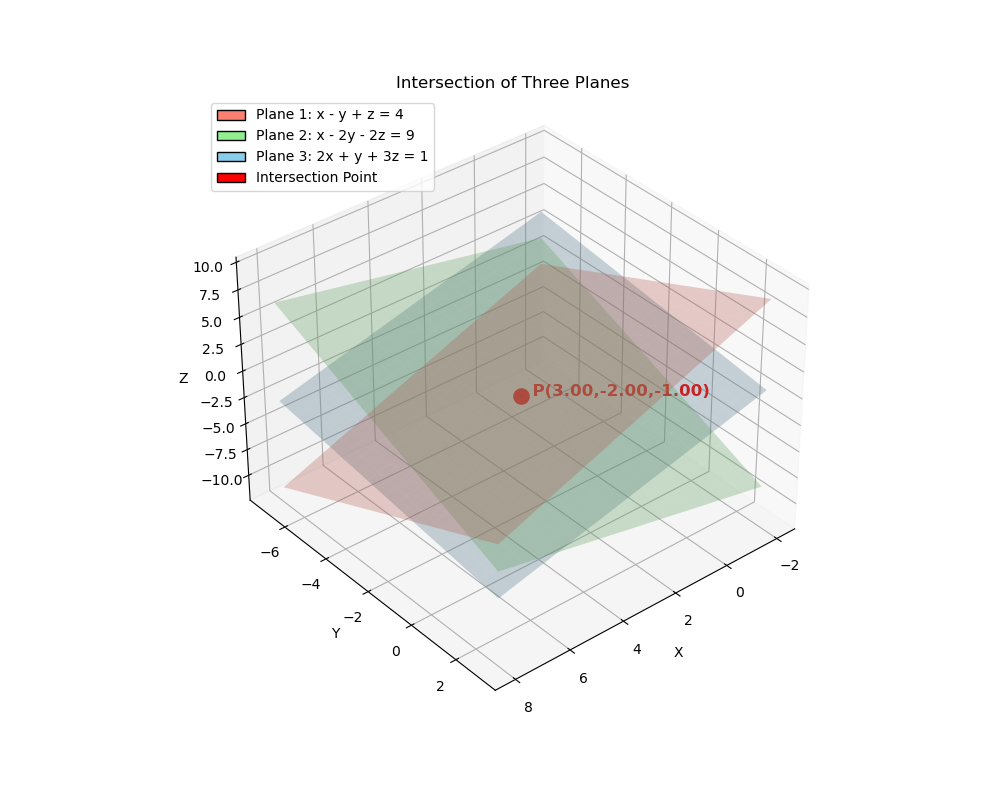
\includegraphics[width=0.5\linewidth]{figures/planes_intersection_c.png}
    \caption{Intersection of three planes}
    \label{fig:placeholder}
\end{figure}



\end{document}
